\begin{figure}
\centering
\begin{subfigure}[b]{0.35\textwidth}
\centering
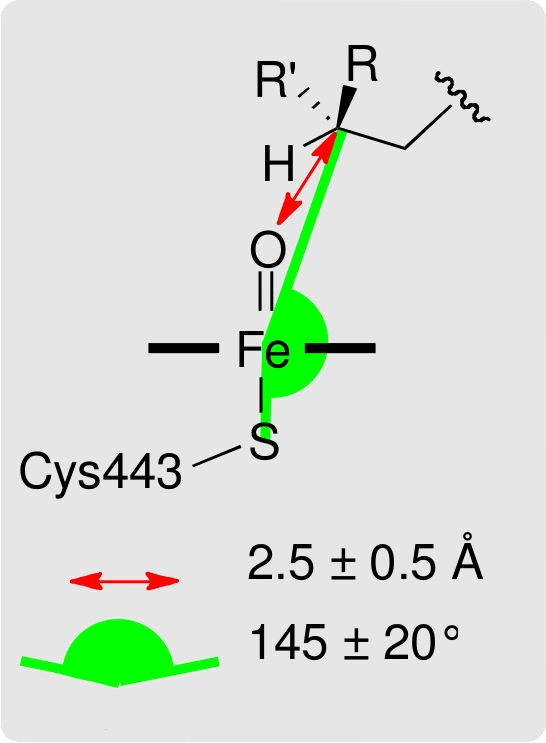
\includegraphics[width=\textwidth]{figures/idsite/33a}
\caption{}
\label{figure:first_sp3_constraints}
\end{subfigure}
\hspace{0.1\textwidth}
\begin{subfigure}[b]{0.35\textwidth}
\centering
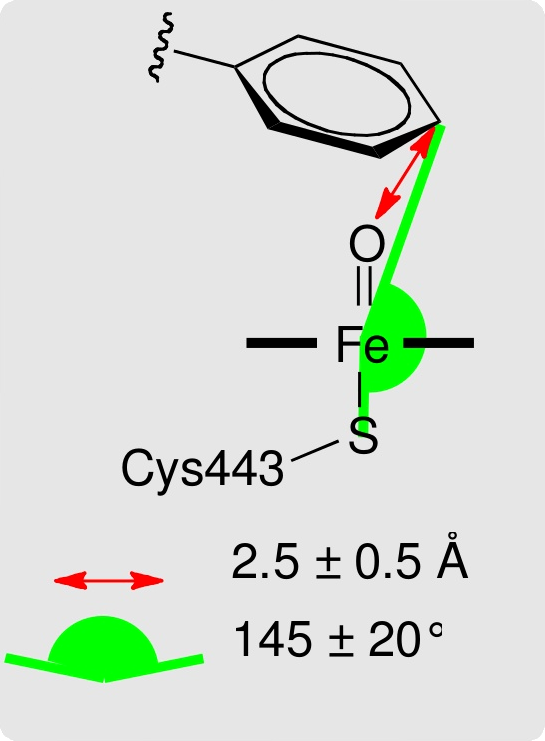
\includegraphics[width=\textwidth]{figures/idsite/33b}
\caption{}
\label{figure:first_sp2_constraints}
\end{subfigure}
\caption{The constraints applied to (a) sp\superscript{3} and (b) sp\superscript{2} atoms during the constrained minimization and first minimization Monte Carlo sampling stage.
The spring constant of the bond constraint (red arrow) is 100 kcal/mol/angstrom\superscript{2}, and that of the angle constraint is 25 kcal/mol/degree\superscript{2}.
The oxygen atom depicted in this figure is a ``dummy'' atom and does not interact with any other atoms in the structure except through the constraint.}
\label{figure:first_constraints}
\end{figure}
